%%%%%%%%%%%%%%%%%%%%%%%%%%%%%%%%%%%%%%%%%%%%%%%%%%%%%%%%%%%%%%%%
%%%%%%%%%%%%%%%%%%%%%%%%%%%%%%%%%%%%%%%%%%%%%%%%%%%%%%%%%%%%%%%%
%%%%
%%%% This text file is part of the source of 
%%%% `Introduction to High-Performance Scientific Computing'
%%%% by Victor Eijkhout, copyright 2012/3/4/5
%%%%
%%%% This book is distributed under a Creative Commons Attribution 3.0
%%%% Unported (CC BY 3.0) license and made possible by funding from
%%%% The Saylor Foundation \url{http://www.saylor.org}.
%%%%
%%%%
%%%%%%%%%%%%%%%%%%%%%%%%%%%%%%%%%%%%%%%%%%%%%%%%%%%%%%%%%%%%%%%%
%%%%%%%%%%%%%%%%%%%%%%%%%%%%%%%%%%%%%%%%%%%%%%%%%%%%%%%%%%%%%%%%

\Level 0 {The idea behind \LaTeX, some history of \TeX}
\index{LaTeX@{\LaTeX}|(}
\index{LaTeX@{\LaTeX}|seealso{\TeX}}
\index{TeX@{\TeX}|(}

\TeX\ is a typesetting system that dates back to the late 1970s. In
those days, graphics terminals where you could design a document layout
and immediately view it, the way you can with for instance Microsoft Word, were
rare.  Instead, \TeX\ uses a two-step workflow, where you first type
in your document with formatting instructions in an ascii document,
using your favourite text editor.
%
Next, you would invoke the
\n{latex} program, as a sort of compiler, to translate this document to
a form that can be printed or viewed. 
\begin{verbatim}
  %% edit mydocument.tex
  %% latex mydocument
  %% # print or view the resulting output
\end{verbatim}
The process is comparable to
making web pages by typing HTML commands.

This way of working may seem clumsy, but
it has some advantages. For instance, the \TeX\ input files are plain
ascii, so they can easily be generated automatically, for instance
from a database. Also, you can edit them with whatever your
favourite editor happens to be.

Another point in favour of \TeX\ is the fact that the layout is
specified by commands that are written in a sort of programming
language. This has some important consequences:
\begin{itemize}
\item Separation of concerns: when you are writing your document, you
  do not have to think about layout. You give the `chapter' command,
  and the implementation of that command will be decided
  independently, for instance by you choosing a document style.
\item Changing the layout of a finished document is easily done by
  choosing a different realization of the layout commands in the input file:
  the same `chapter' command is used, but by choosing a different
  style the resulting layout is
  different. This sort of change can be as simple as 
  a one-line change to the document style declaration.
\item If you have unusual typesetting needs, it is possible to write
  new \TeX\ commands for this. For many needs such extensions have in
  fact already been written; see section~\ref{sec:moreLaTeX}.
\end{itemize}

The commands in \TeX\ are fairly low level. For this reason, a number
of people have written systems on top of \TeX\ that offer powerful
features, such as automatic cross-referencing, or generation of a
table of contents. The most popular of these systems is \LaTeX. Since
\TeX\ is an interpreted system, all of its mechanisms are still
available to the user, even though \LaTeX\ is loaded on top of it.

\index{TeX@{\TeX}|)}

\Level 1 {Installing \LaTeX}

The easiest way to install \LaTeX\ on your system is by downloading
the \TeX{}live distribution from \url{http://tug.org/texlive}. Apple
users can also use \n{fink} or \n{macports}. Various front-ends to
\TeX\ exist, such as \TeX{}shop on the Mac.

\Level 1 {Running \LaTeX}

\begin{purpose}
In this section you will run the \LaTeX\ compiler  
\end{purpose}

Originally, the \n{latex} compiler would output a device independent
file format, named \n{dvi}, which could then be translated to
PostScript or PDF, or directly printed. These days, many people use
the \n{pdflatex} program which directly translates \n{.tex} files to
\n{.pdf} files. This has the big advantage that the generated PDF
files have automatic cross linking and a side panel with table of
contents. An illustration is found below.

Let us do a simple example.
\begin{figure}[ht]
\begin{verbatim}
\documentclass{article}
\begin{document}
Hello world!
\end{document}
\end{verbatim}
  \caption{A minimal \LaTeX\ document}
  \label{fig:minimaldoc}
\end{figure}
\practical
{Create a text file \n{minimal.tex} with the content as in
  figure~\ref{fig:minimaldoc}. Try the command \n{pdflatex minimal} or
  \n{latex minimal}. Did you get a file \n{minimal.pdf} in the first
  case or \n{minimal.dvi} in the second case? Use a pdf viewer, such
  as Adobe Reader, or
  \n{dvips} respectively to view the output.}  
{}
{If you make a typo, \TeX\ can be somewhat unfriendly. If you get an
  error message and \TeX\ is asking for input, typing \n{x}
  usually gets you out, or \n{Ctrl-C}. Some systems allow you to type
  \n{e} to go directly into the editor to correct the typo.}

\Level 0 {A gentle introduction to LaTeX}

Here you will get a very brief run-through of \LaTeX\ features. There
are various more in-depth tutorials available, such as the one by
Oetiker~\cite{Oetiker:LaTeXintro}.

\Level 1 {Document structure}

Each \LaTeX\ document needs the following lines:
\begin{verbatim}
  \documentclass{ .... } % the dots will be replaced

  \begin{document}

  \end{document}  
\end{verbatim}
The `documentclass' line needs a class name in between the braces;
typical values are `article' or `book'. Some organizations have their
own styles, for instance `ieeeproc' is for proceedings of the IEEE.

All document text goes between the \verb+\begin{document}+ and
\verb+\end{document}+ lines. (Matched `begin' and `end' lines are said
to denote an `environment', in this case the document environment.)

The part before \verb+\begin{document}+ is called the `preamble'. It
contains customizations for this particular document. For instance, a
command to make the whole document double spaced would go in the
preamble. If you are using \n{pdflatex} to format your document, you
want a line
\begin{verbatim}
  \usepackage{hyperref}
\end{verbatim}
here.

Have you noticed the following?
\begin{itemize}
\item The backslash character is special: it starts a \LaTeX\ command.
\item The braces are also special: they have various functions, such
  as indicating the argument of a command.
\item The percent character indicates that everything to the end of
  the line is a comment.
\end{itemize}

\Level 1 {Some simple text}

\begin{purpose}
  In this section you will learn some basics of text formatting.
\end{purpose}

\practical
{Create a file \n{first.tex} with the content of
  figure~\ref{fig:minimaldoc} in it. Type some text in the preamble,
  that is, before the
  \n{\\begin\{document\}} line and run \n{pdflatex} on your file.}
{You should get an error message because you are not allowed to have text
  in the preamble. Only commands are allowed there; all text has to go after
  \n{\\begin\{document\}}.}{}

\practical
{Edit your document: put some text in between the 
\n{\\begin\{document\}} and \n{\\end\{document\}} lines.
Let your text have both some long lines that go on for a while,
and some short ones. Put superfluous spaces between words, and at the
beginning or end of lines. Run \n{pdflatex} on your document and view
the output.}
{You notice that the white space in your input has been collapsed in the
  output. \TeX\ has its own notions about what space should look like,
  and you do not have to concern yourself with this matter.}{}

\practical 
{Edit your document again, cutting and pasting the
  paragraph, but leaving a blank line between the two copies. Paste it
  a third time, leaving several blank lines. Format, and view the
  output.}
{\TeX\ interprets one or more blank lines as the
  separation between paragraphs.}{}

\practical
{Add \n{\\usepackage\{pslatex\}} to the preamble and rerun
  \n{pdflatex} on your
document. What changed in the output?}
{This should have the effect of changing the typeface from the default
  to Times Roman.}
{Typefaces are notoriously unstandardized. Attempts to use different
  typefaces may or may not work. Little can be said about this in general.}

Add the following line before the first paragraph:
\begin{verbatim}
  \section{This is a section}
\end{verbatim}
and a similar line before the
second. Format. You see that \LaTeX\ automatically numbers the
sections, and that it handles indentation different for the first
paragraph after a heading.

\practical
{Replace \n{article} by \n{artikel3} in the documentclass declaration line and
reformat your document. What changed?}
{There are many documentclasses that implement the same commands as
  \n{article} (or another standard style), but that have their own
  layout. Your document should format without any problem, but get a
  better looking layout.}
{The \n{artikel3} class is part of most distributions these days, but
  you can get an error message about an unknown documentclass if it is
  missing or if your environment is not set up correctly. This depends
  on your installation. If the file seems missing, download the files
  from \url{http://tug.org/texmf-dist/tex/latex/ntgclass/}
  and put them in your current directory; see also section~\ref{sec:texinputs}.}

\Level 1 {Math}

\begin{purpose}
  In this section you will learn the basics of math typesetting
\end{purpose}

One of the goals of the original \TeX\ system was to facilitate the
setting of mathematics. There are two ways to have math in your
document:
\begin{itemize}
\item Inline math is part of a paragraph, and is delimited by dollar
  signs. 
\item Display math is, as the name implies, displayed by itself. 
\end{itemize}

\practical
{Put \n{\$x+y\$} somewhere in a paragraph and format your document.
Put  \n{\\[x+y\\]} somewhere in a paragraph and format.}
{Formulas between single dollars are included in the paragraph where
  you declare them. Formulas between \n{\\[...\\]} are typeset in a
  display.}
{}

For display
equations with a number, use an \n{equation} environment. Try this.

Here are some common things to do in math. Make sure to try them out.
\begin{itemize}
\item Subscripts and superscripts: \verb-$x_i^2$-. If the sub or superscript
  is more than a single symbol, it needs to be grouped:
  \verb-$x_{i+1}^{2n}$-. If you need a brace in a formula, use
  \verb-$\{ \}$-.
\item Greek letters and other symbols: \verb-$\alpha\otimes\beta_i$-.
\item Combinations of all these \verb-$\int_{t=0}^\infty tdt$-.
\end{itemize}

\practical{Take the last example and typeset it as display math. Do
  you see a difference with inline math?}
{\TeX\ tries not to include the distance between text lines, even if
  there is math in a paragraph. For this reason it typesets the bounds
  on an integral sign differently from display math.}{}

\Level 1 {Referencing}

\begin{purpose}
  In this section you will see \TeX's cross referencing mechanism in action.
\end{purpose}

So far you have not seen \LaTeX\ do much that would save you any
work. The cross referencing mechanism of \LaTeX\ will definitely save
you work: any counter that \LaTeX\ inserts (such as section numbers)
can be referenced by a label. As a result, the reference will always
be correct.

Start with an example
document that has at least two section headings. After your first section
heading, put the command \verb+\label{sec:first}+,
and put \verb+\label{sec:other}+ after the second section
heading. These label commands can go on the same line as the
\n{section} command, or on the next.
Now put 
\begin{verbatim}
  As we will see in section~\ref{sec:other}.
\end{verbatim}
in the paragraph before the second section. (The tilde character
denotes a non-breaking space.) 

\practical{Make these edits and format the document. Do
you see the warning about an undefined reference? Take a look at the
output file. Format the document
again, and check the output again.
Do you have any new files in your directory?}
{On a first pass through a document, the \TeX\ compiler will gather
  all labels with their values in a \n{.aux} file. The document will
  display a double question mark for any references that are
  unknown. In the second pass the correct values will be filled
  in.}
{If after the second pass there are still undefined references, you
  probably made a typo. If you use the \n{bibtex} utility for
  literature references, you will regularly need three passes to get
  all references resolved correctly.}

Above you saw that the \n{equation} environment gives displayed
math with an equation number. You can add a label to this environment
to refer to the equation number.

\practical{Write a formula in an \n{equation}
environment, and add a label.  Refer to this label anywhere in the
text. Format (twice) and check the output.}
{The \n{\\label} and \n{\\ref} command are used in the same way for
  formulas as for section numbers. Note that you must use
  \n{\\begin/end\{equation\}} rather than \n{\\[...\\]} for the formula.}{}

\Level 1 {Lists}

\begin{purpose}
  In this section you will see the basics of lists.
\end{purpose}

Bulleted and numbered lists are provided through an environment.
\begin{verbatim}
\begin{itemize}
\item This is an item;
\item this is one too.
\end{itemize}
\begin{enumerate}
\item This item is numbered;
\item this one is two.
\end{enumerate}
\end{verbatim}

\practical{Add some lists to your document, including nested
  lists. Inspect the output.}
{Nested lists will be indented further and the labeling and numbering
  style changes with the list depth.}{}

\practical{Add a label to an item in an \n{enumerate} list and refer
  to it.}
{Again, the \n{\\label} and \n{\\ref} commands work as before.}{}

\Level 1 {Source code and algorithms}

As a computer scientist, you will often want to include 
algorithms in your writings; sometimes even source code.

In this tutorial so far you have seen that some characters
have special meaning to \LaTeX{}, and just can not just type them
and expect them to show up in the output. Since funny characters
appear quite regularly in programming languages, we need a tool for this:
the \indexterm{verbatim mode}.

To display bits of code inside a paragraph, you use the \verb+\verb+
command.  This command delimits its argument with two identical
characters that can not appear in the verbatim text. For instance,
the output
\verb+if (x%5>0) { ... }+ is produced by \verb/\verb+if (x%5>0) { ... }+/.
(Exercise: how did the author of this book get that verbatim command
in the text?)

For longer stretches of verbatim text, that need to be displayed
by themselves you use
\begin{quote}
\leavevmode\noindent\parindent=0pt
\hbox{\verb+\begin{verbatim}+}\\
\hbox{\verb+stuff+}\\
\hbox{\verb+\end{verbatim}+}
\end{quote}
Finally, in order to include a whole file as verbatim listing, use
\n{\verbatiminput{path/filename}}.

Verbatim text is one way of displaying algorithms, but there are
more elegant solutions. For instance, in this book the following is
used:
\begin{verbatim}
\usepackage[algo2e,noline,noend]{algorithm2e}
\end{verbatim}
The result can be seen, for instance, on page~\pageref{fig:taskqueue}.

\Level 1 {Graphics}

Since you can not immediately see the output of what you are typing,
sometimes the output may come as a surprise. That is especially so
with graphics. \LaTeX\ has no standard way of dealing with graphics,
but the following is a common set of commands:
\begin{verbatim}
\usepackage{graphicx} % this line in the preamble

\includegraphics{myfigure} % in the body of the document
\end{verbatim}
The figure can be in any of a number of formats, except that
PostScript figures (with extension \n{.ps} or \n{.eps})
can not be used if you use pdflatex.

Since your figure is often not the right size, the include line will
usually have something like:
\begin{verbatim}
\includegraphics[scale=.5]{myfigure}  
\end{verbatim}
A bigger problem is that figures can be too big to fit on the page if
they are placed where you declare them. For this reason, they are
usually treated as `floating material'. Here is a typical  declaration
of a figure:
\begin{verbatim}
\begin{figure}[ht]
  \includegraphics{myfigure}
  \caption{This is a figure}
  \label{fig:first}
\end{figure}
\end{verbatim}
It contains the following elements:
\begin{itemize}
\item The \n{figure} environment is for `floating' figures; they can
  be placed right at the location where they are declared, at the top
  or bottom of the next page, at the end of the chapter, et cetera.
\item The \n{[ht]} argument of the \n{\\begin\{figure\}} line
  states that your figure should be attempted to be placed \n{h}ere; it
  that does not work, it should go \n{t}op of the next page. The
  remaining possible specifications are \n{b} for placement at the bottom of a
  page, or \n{p}~for placement on a page by itself. For example
\begin{verbatim}
  \begin{figure}[hbp]
\end{verbatim}
  declares that the figure has to be placed here if possible, at the
  bottom of the page if that's not possible, and on a page of its
  own if it is too big to fit on a page with text.
\item A caption to be put under the figure, including a figure number;
\item A label so that you can refer to the figure number by its label:
  \n{figure\char`\~\\ref\{fig:first\}}.
\item And of course the figure material. There are various ways to
  fine-tune the figure placement. For instance
\begin{verbatim}
  \begin{center}
    \includegraphics{myfigure}
  \end{center}
\end{verbatim}
  gives a centered figure.
\end{itemize}

\Level 1 {Bibliography references}
\label{sec:bib-latex}

The mechanism for citing papers and books in your document is a bit
like that for cross referencing. There are labels involved, and there
is a \verb+\cite{thatbook}+ command that inserts a reference, usually
numeric. However, since you are likely to refer to a paper or book in
more than one document your write, \LaTeX\ allows you to have a
database of literature references in a file by itself,
rather than somewhere in your document.

Make a file \n{mybibliography.bib} with the following content:
\begin{verbatim}
@article{JoeDoe1985,
author = {Joe Doe},
title = {A framework for bibliography references},
journal = {American Library Assoc. Mag.},
year = {1985}
}
\end{verbatim}
In your document \n{mydocument.tex}, put
\begin{verbatim}
For details, refer to Doe~\cite{JoeDoe1985} % somewhere in the text

\bibliography{mybibliography} % at the end of the document
\bibliographystyle{plain}
\end{verbatim}
Format your document, then type on the commandline
\begin{verbatim}
bibtex mydocument
\end{verbatim}
and format your document two more times. There should now be a
bibliography in it, and a correct citation. You will also see that
files \n{mydocument.bbl} and \n{mydocument.blg} have been created.

\Level 1 {Environment variables}
\label{sec:texinputs}
\index{TeX@{\TeX}!environment variables|(}

On Unix systems, \TeX\ investigates the \n{TEXINPUTS} \emph{environment
variable} when it tries to find an include file. Consequently, you can
create a directory for your styles and other downloaded include files,
and set this variable to the location of that directory.
Similarly, the \n{BIBINPUTS} variable indicates the location of
bibliography files for bibtex (section~\ref{sec:bib-latex}).

\index{TeX@{\TeX}!environment variables|)}

\Level 0 {A worked out example}

The following example \n{demo.tex} contains many of the elements discussed above.

\begingroup\small
\verbatiminput{tutorials/latexdemo/demo.tex}
\endgroup

You also need the file \n{math.bib}:

\begingroup\small
\verbatiminput{tutorials/latexdemo/math.bib}
\endgroup

The following sequence of commands
\begin{verbatim}
  pdflatex demo
  bibtex demo
  pdflatex demo
  pdflatex demo
\end{verbatim}
gives 

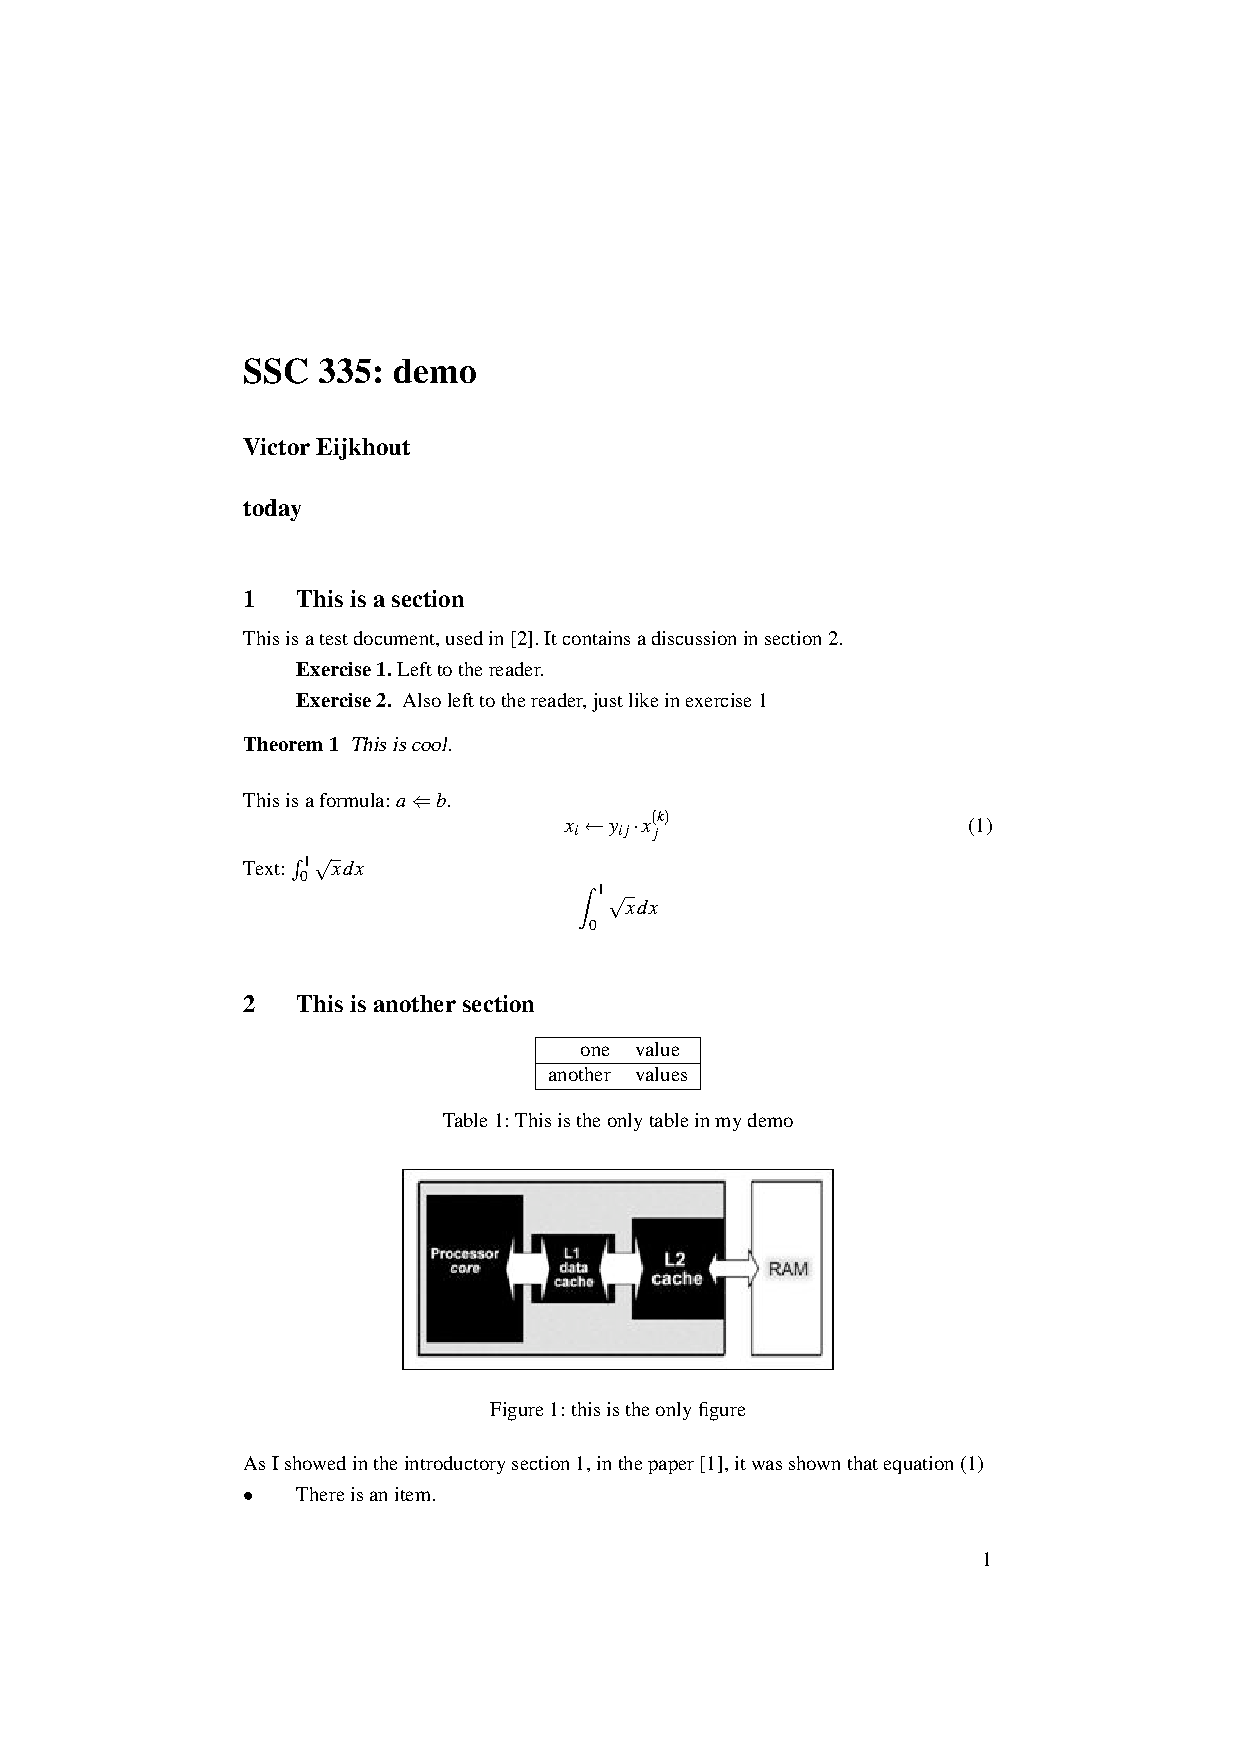
\includegraphics[scale=.75]{tutorials/latexdemo/demopage1}

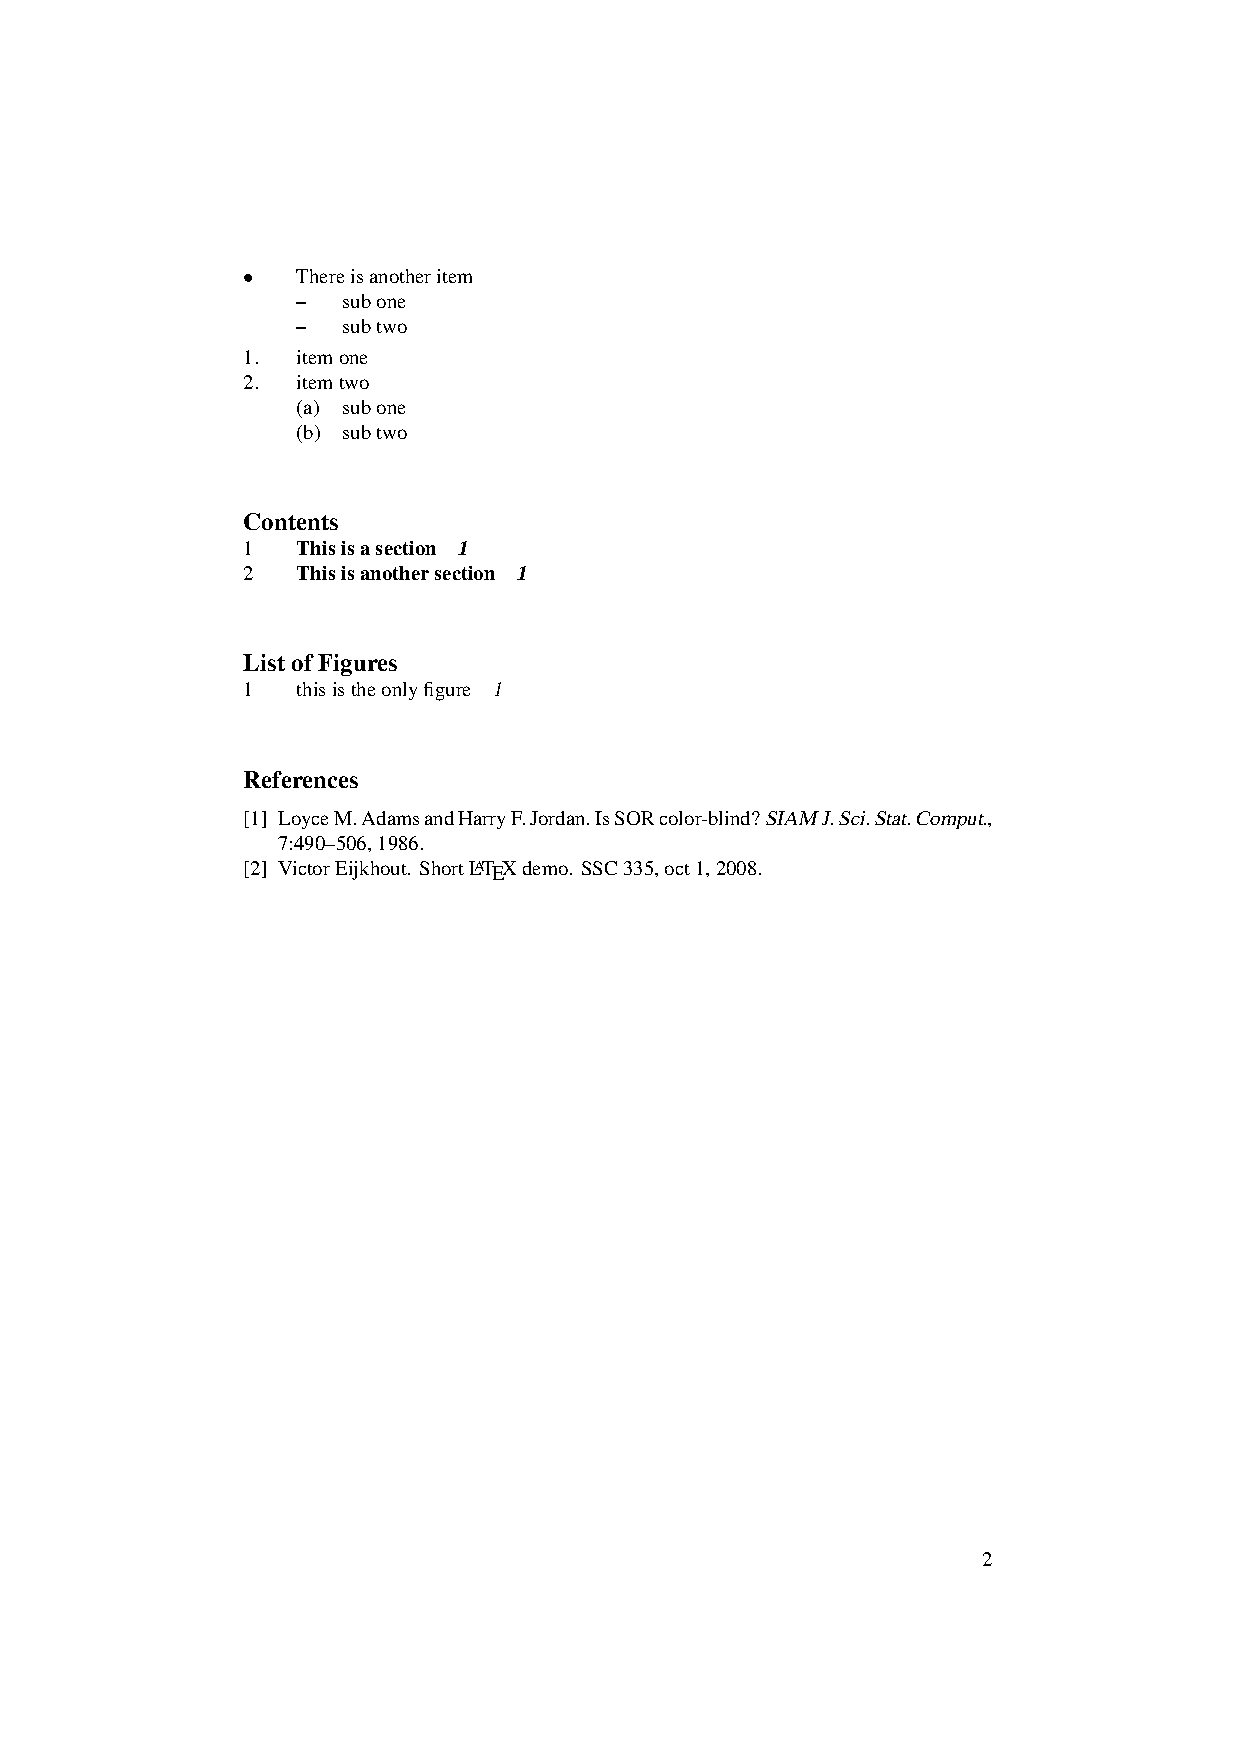
\includegraphics[scale=.75]{tutorials/latexdemo/demopage2}

\Level 0 {Where to take it from here}
\label{sec:moreLaTeX}

This tutorial touched only briefly on some essentials of \TeX\ and
\LaTeX. You can find longer intros online~\cite{Oetiker:LaTeXintro},
or read a book~\cite{Lamport:LaTeX,KopkaDaly,LaTeXcompanion}. Macro
packages and other software can be found on the Comprehensive
\TeX\ Archive \url{http://www.ctan.org}. For questions you can go to
the newsgroup \n{comp.text.tex}, but the most common ones can often
already be found on web sites~\cite{UKTeXFAQ}.

\begin{istc}
  
\Level 0 {Review questions}

\begin{exercise}
Write a one or two page document about your field of study. Show that
you have mastered the following constructs:
\begin{itemize}
\item formulas, including labels and referencing;
\item including a figure;
\item using bibliography references;
\item construction of nested lists.
\end{itemize}

\end{exercise}

\end{istc}

\index{LaTeX@{\LaTeX}|)}
